%15 min preso!
\documentclass[xcolor=table,aspectratio=169,fleqn]{beamer}
\usepackage{beamerthemesplit}
\usepackage{wrapfig}
\usetheme{SPbGU}
\usepackage{pdfpages}
\usepackage{amsmath}
\usepackage{mathtools}
\usepackage{cmap}
\usepackage[T2A]{fontenc}
\usepackage[utf8]{inputenc}
\usepackage[english]{babel}
\usepackage{indentfirst}
\usepackage{newtxmath}
\usepackage{tikz}
\usepackage{multirow}
\usepackage[noend]{algpseudocode}
\usepackage{algorithm}
\usepackage{algorithmicx}
\usepackage{fancyvrb}
\usepackage{hyperref}
\usepackage{nicematrix}
\definecolor{links}{HTML}{2A1B81}
\hypersetup{colorlinks,linkcolor=,urlcolor=links}
\usetikzlibrary{calc}
\usetikzlibrary{shapes, backgrounds}
\usetikzlibrary{arrows,automata}
\usetikzlibrary{positioning}
\usetikzlibrary{fit}
\usetikzlibrary{shapes.callouts}
\usetikzlibrary{shapes.misc}
\usepackage{xparse}
\usepackage{fontawesome}

\usepackage{etoolbox,refcount}
\usepackage{multicol}

\usepackage{tabularx}
\newcolumntype{Y}{>{\raggedleft\arraybackslash}X}

\renewcommand{\thealgorithm}{}

\newtheorem{mytheorem}{Theorem}
\renewcommand{\thealgorithm}{}

\newcommand{\tikzmark}[1]{\tikz[overlay,remember picture] \node (#1) {};}
\def\Put(#1,#2)#3{\leavevmode\makebox(0,0){\put(#1,#2){#3}}}

\newcommand{\ltz}{$< 1$}

\tikzset{
    state/.style={
           rectangle,
           rounded corners,
           draw=black, very thick,
           minimum height=1.5em,
           inner sep=2pt,
           text centered,
           },
}

\tikzset{
    invisible/.style={opacity=0,text opacity=0},
    visible on/.style={alt=#1{}{invisible}},
    alt/.code args={<#1>#2#3}{%
      \alt<#1>{\pgfkeysalso{#2}}{\pgfkeysalso{#3}} % \pgfkeysalso doesn't change the path
    },
}

\tikzset{cross/.style={cross out, draw=black, minimum size=2*(#1-\pgflinewidth), inner sep=0pt, outer sep=0pt, ultra thick},
%default radius will be 1pt. 
cross/.default={1pt}}

\NewDocumentCommand{\mycallout}{r<> O{opacity=0.8,text opacity=1} m m m}{%
\tikz[remember picture, overlay]\node[align=center, fill=cyan!20, text width=#5cm,
#2,visible on=<#1>, rounded corners,
draw,rectangle callout,anchor=pointer,callout relative pointer={(290:0.5cm)}]
at (#3) {#4};
}

\NewDocumentCommand{\mycalloutR}{r<> O{opacity=0.8,text opacity=1} m m m}{%
\tikz[remember picture, overlay]\node[align=center, fill=cyan!20, text width=#5cm,
#2,visible on=<#1>, rounded corners,
draw,rectangle callout,anchor=pointer,callout relative pointer={(30:0.8cm)}]
at (#3) {#4};
}

\newcommand\colR{\cellcolor{red!20}}
\newcommand\colB{\cellcolor{blue!20}}
\newcommand\colG{\cellcolor{green!20}}
\newcommand\colO{\cellcolor{orange!20}}
\definecolor{Gray}{gray}{0.8}

%callout relative pointer={(230:0.5cm)}]

\newcounter{countitems}
\newcounter{nextitemizecount}
\newcommand{\setupcountitems}{%
  \stepcounter{nextitemizecount}%
  \setcounter{countitems}{0}%
  \preto\item{\stepcounter{countitems}}%
}
\makeatletter
\newcommand{\computecountitems}{%
  \edef\@currentlabel{\number\c@countitems}%
  \label{countitems@\number\numexpr\value{nextitemizecount}-1\relax}%
}
\newcommand{\nextitemizecount}{%
  \getrefnumber{countitems@\number\c@nextitemizecount}%
}
\newcommand{\previtemizecount}{%
  \getrefnumber{countitems@\number\numexpr\value{nextitemizecount}-1\relax}%
}
\makeatother    
\newenvironment{AutoMultiColItemize}{%
\ifnumcomp{\nextitemizecount}{>}{3}{\begin{multicols}{2}}{}%
\setupcountitems\begin{itemize}}%
{\end{itemize}%
\unskip\computecountitems\ifnumcomp{\previtemizecount}{>}{3}{\end{multicols}}{}}


\beamertemplatenavigationsymbolsempty


\title[Линейная алгебра, формальные зыки и графы]{Анализ графов с использованием формальных языков в качестве ограничений на пути}
\subtitle{Заготовки для докторской диссертации}
\institute[СПбГУ]{
Санкт-Петербургский Государственный Университет
}

\author[Семён Григорьев]{Семён Григорьев}

\date{!!! !!!! 2026}

\begin{document}
{
\begin{frame}[fragile]
  \begin{table}
  \centering  
  \begin{tabularx}{\linewidth}{XcX}
    \hfill
    & 
    & \hfill \includegraphics[height=1.4cm]{pictures/SPbSU_Logo.pdf}
  \end{tabularx}
  \end{table}
  \titlepage
\end{frame}
}


\begin{frame}[fragile]
  \frametitle{Формальные языки и ограничения на пути в графе}
  \begin{minipage}{0.2\textwidth}
    \begin{tikzpicture}[shorten >=1pt,auto]
      \node[state] (q_0)                      {$0$};
      \node[state] (q_1) [above right=of q_0] {$1$};
      \node[state,fill=red!20] (q_2) [right=of q_0]       {$2$};
      \node[state] (q_3) [right=of q_2]       {$3$};
      \path[->]
      (q_0) edge  node {a} (q_1)
      (q_1) edge  node {a} (q_2)
      (q_2) edge  node {a} (q_0)
      (q_2) edge[bend left, above]  node {b} (q_3)
      (q_3) edge[bend left, below]  node {b} (q_2);
    \end{tikzpicture}
  \end{minipage}
  \begin{minipage}{0.75\textwidth}    
    \begin{itemize}
      \item $G = \langle V, E, L \rangle$ --- (ориентированный) граф с метками на рёбрах
      \item Путь $\pi$ задаёт слово: $\omega(_2 \pi_1) = \omega(2 \xrightarrow{a} 0 \xrightarrow{a} 1) = aa$
      \item Ищем пути, задающие слова определённого вида
      \begin{itemize} 
        \item Например, слова вида $a^*b$
      \end{itemize} 
      \item Множество слов --- язык $\mathcal{L}$ над алфавитом $\Sigma$
      \begin{itemize} 
        \item Для удобства будем считать, что $\Sigma \cap L \neq \varnothing$
      \end{itemize} 
    \end{itemize}
  \end{minipage}
  \vfill
  \pause
  \begin{block}{Варианты задач \textbf{\underline{Formal Language Constrained Path Quering} (FLPQ)}}
    Для данного графа $G$, стартовых вершин $V_s \in V$ и финальных вершин $V_f \in V$, языка $\mathcal{L}$ 
    \begin{itemize}
      \pause
      \item Задача достижимости: $R = \{ (u,v) \mid \omega(_u\pi_v) \in \mathcal{L}, u \in V_s, v \in V_f \}$
      \pause
      \item Задача поиска всех путей: $P = \{ \pi \mid \omega(_u\pi_v) \in \mathcal{L}, u \in V_s, v \in V_f \}$
      \pause
      \item Задача поиска одного пути
      \item Задача проверки наличия достижимых пар
    \end{itemize}
  \end{block}

\end{frame}

\begin{frame}[fragile]
  \frametitle{Области применения}
  \begin{itemize}
    \item Регулярные языки
    \begin{itemize}
      \item Графовые базы данных (Regular Path Queries, RPQ), ISO, !!!!
      \item Параметризация алгебраическими структурами: полукольцами, моноидами и т.д.
    \end{itemize}
    \pause
    \item Контекстно-свободные языки
    \begin{itemize}
      \item Статический анализ кода, унификация !!!
      \item Графовые базы данных
      \item !!!
    \end{itemize}
    \pause
    \item За пределами контекстно-свободных
    \begin{itemize}
      \item Многокомпонентные контекстно-свободные !!!
      \item Линейные конъюнктивные !!!
    \end{itemize}
  \end{itemize}
\end{frame}

\begin{frame}[fragile]
  \frametitle{Состояние дел}
  \begin{itemize}
    \item API для создания алгоритмов анализа графов на основе линейной алгебры 
    \begin{itemize}
      \item Различные операции над матрицами и векторами (\underline{\textbf{разреженными}})
      \item Параметризация алгебраическими структурами: полукольцами, моноидами и т.д.
    \end{itemize}
    \pause
    \item Позволяет выражать \underline{\textbf{различные}} алгоритмы
    \begin{itemize}
      \item Обход в ширину, поиск кратчайших путей, достижимость, \ldots
      \item Подсчёт треугольников, PageRank, остовные деревья, кластеризация, \ldots
      \item Навигационные запросы: \textbf{RPQ, CFPQ,} \ldots
    \end{itemize}
    \pause
    \item Подробнее
    \begin{itemize}
      %\item The GraphBLAS C API Specification\footnote{\url{https://graphblas.org/docs/GraphBLAS_API_C_v2.1.0.pdf}}
      \item GraphBLAS Pointers\footnote{\url{https://graphblas.org/GraphBLAS-Pointers/}}
      \item \textbf{SuiteSparse:GraphBLAS}\footnote{\url{https://github.com/DrTimothyAldenDavis/GraphBLAS}} --- \underline{\textbf{эталон}} на чистом C
      \item \textbf{LAGraph}\footnote{\url{https://github.com/GraphBLAS/LAGraph}} --- коллекция \underline{\textbf{прикладных}} алгоритмов анализа графов
    \end{itemize}
    \end{itemize}
\end{frame}

\begin{frame}[fragile]
  \frametitle{Проблемы}
  \vspace{-0.3cm}
  \begin{minipage}[t]{0.49\textwidth}
    \onslide<1->{
    $R_1 = \{(\textcolor{blue}{a},\textcolor{red}{y});(\textcolor{blue}{b},\textcolor{red}{x});(\textcolor{blue}{b},\textcolor{red}{z})\}$\\
  $R_2 = \{(\textcolor{red}{x},\textcolor{green}{u});(\textcolor{red}{x},\textcolor{green}{w});(\textcolor{red}{y},\textcolor{green}{v});(\textcolor{red}{y},\textcolor{green}{w});(\textcolor{red}{z},\textcolor{green}{u})\}$\\
    }
  \onslide<2->{
  $R_3 = \{ (i,j) \mid (i,k) \in R_1, (k,j) \in R_2 \}$
    }
  \\  
  \vspace{-0.4cm}
      \NiceMatrixOptions{code-for-first-row = \color{red},
                     code-for-first-col = \color{blue},
                     code-for-last-row = \color{red},
                     code-for-last-col = \color{blue}}
\onslide<3->{
$$
\begin{pNiceArray}{ccc}[first-col,first-row,nullify-dots]
  & x & y & z \\
a & 0 & 1 & 0 \\
b & 1 & 0 & 1 \\
\end{pNiceArray}
\times
\NiceMatrixOptions{code-for-first-row = \color{green},
                     code-for-first-col = \color{red}}
\begin{pNiceArray}{ccc}[first-col,first-row,nullify-dots]
    & u & v & w \\
  x & 1 & 0 & 1 \\
  y & 0 & 1 & 1 \\
  z & 1 & 0 & 0 \\
\end{pNiceArray}
=
\NiceMatrixOptions{code-for-first-row = \color{green},
                     code-for-first-col = \color{blue}}
\begin{pNiceArray}{ccc}[first-col,first-row,nullify-dots]
    & u & v & w \\
  a & 0 & 1 & 1 \\
  b & 1 & 0 & 1 \\  
\end{pNiceArray}
$$
}
\vspace{-0.4cm}
\onslide<4->{
\begin{center}
\begin{tikzpicture}[shorten >=1pt,auto]
    \node[state,fill=blue!20] (q_0)                      {$a$};
    \node[state,fill=blue!20] (q_1) [below = of q_0 ]    {$b$};

    \node[state,fill=red!20] (q_2)  [right = of q_0 ]    {$x$};
    \node[state,fill=red!20] (q_3)  [right = of q_1 ]    {$y$};
    \node[state,fill=red!20] (q_4)  [below = of q_3 ]    {$z$};
    
    \node[state,fill=green!20] (q_5)  [right = of q_2 ]    {$u$};
    \node[state,fill=green!20] (q_6)  [right = of q_3 ]    {$v$};
    \node[state,fill=green!20] (q_7)  [right = of q_4 ]    {$w$};

    \onslide<5->
{
    \path[->]
    (q_0) edge  node {} (q_3)
    (q_1) edge  node {} (q_2)
    (q_1) edge  node {} (q_4);
}
\onslide<6->
{
     \path[->]    
    (q_2) edge  node {} (q_5)
    (q_2) edge  node {} (q_7)
    (q_3) edge  node {} (q_6)
    (q_3) edge  node {} (q_7)
    (q_4) edge  node {} (q_5);
}
\onslide<7->
{
 \path[->,red]
   (q_0) edge  node {} (q_6)
   (q_0) edge[bend right=20]  node {} (q_7)
   (q_1) edge  node {} (q_5)
   (q_1) edge[bend right=10]  node {} (q_7)
   ;
}
\end{tikzpicture}
\end{center}
}
  \end{minipage}
  \begin{minipage}[t]{0.45\textwidth}
    \onslide<1->{
    \scriptsize{
    \begin{flalign*}
     &|S_A| = n, |S_B| = k, |S_C| = m  \\
     &\mathcal{N_A}: [0\ldots (n-1)] \to S_A,\text{ биекция} \\
     &\mathcal{N_B}: [0\ldots (k-1)] \to S_B,\text{ биекция} \\
     &\mathcal{N_C}: [0\ldots (m-1)] \to S_C,\text{ биекция} \\
     & R_1 \subseteq S_A \times S_B, R_2 \subseteq S_B \times S_C \\     
     & R_3 = \{ (x,z) \mid (x,y) \in R_1, (y,z) \in R_2 \} \\
     & M_{n \times k}^{R_1} = 1 \iff (\mathcal{N_A}(i),\mathcal{N_B}(j)) \in R_1 \text{, иначе } M^{R_1} = 0 \\
     & M_{k \times m}^{R_2} = 1 \iff (\mathcal{N_B}(i),\mathcal{N_C}(j)) \in R_2 \text{, иначе } M^{R_2} = 0 \\
     & M_{n \times m}^{R_3} = M^{R_1} \times M^{R_2}
    \end{flalign*}
    }    
    }
  \end{minipage}
\end{frame}


\begin{frame}[fragile]
  \frametitle{Цель работы}
  Целью диссертационной работы является создание общей методологии анализа графов с использованием формальных языков в качестве ограничений на пути. Для её достижения необходимо решить следующие задачи.
Провести систематизацию имеющихся результатов, с одной стороны, для выявления мест, требующих более детального изучения и формализации, а с другой, для обнаружения общих закономерностей, позволяющих построить общее описание рассматриваемой области. В частности, необходимо изучить существующие алгоритмы решения задачи анализа графов с использованием формальных языков в качестве ограничений на пути. Кроме этого, необходимо провести анализ областей применения, выявление характерных особенностей задач, возникающих в них, выявить и структурировать основные требования к применяемым в данных областях алгоритмам. 
Разработать методологию анализа графов с использованием формальных языков в качестве ограничений на пути, предоставляющую средства для классификации задач, включающую методы построения и анализа алгоритмов решения соответствующих задач. 
Разработать метод создания алгоритмов, в том числе параллельных, на основе линейной алгебры для решения задач анализа графов с использованием формальных языков в качестве ограничений на пути. Проверить метод на практике, создав семейство соответствующих алгоритмов.
Разработать метод создания алгоритмов на основе классических алгоритмов синтаксического анализа. Проверить метод на практике, создав семейство соответствующих алгоритмов.
Разработать методику проведения экспериментального исследования алгоритмов анализа графов, использующих формальные языки в качестве ограничений на пути. В том числе, создать набор данных для проведения экспериментов, разработать архитектуру необходимой инфраструктуры.
Исследовать применимость разработанных алгоритмов к решению прикладных задач, спроектировать и реализовать соответствующие библиотеки и инструментальные средства.
Разработать методические рекомендации по выстраиванию междисциплинарных связей, необходимых для лучшего понимания задач анализа графов с использованием формальных языков в качестве ограничений на пути и областей их применения.




\end{frame}


\begin{frame}[fragile]
  \frametitle{Положения, выносимые на защиту}
  \begin{enumerate}[<+->]
    \item Создана методология анализа графов с использованием формальных языков в качестве ограничений на пути, нацеленная на конструирование алгоритмов FLPQ    
    \item Разработаны методы конструирования алгоритмов решения FLPQ
    \begin{itemize} 
      \item Использующих операции линейной алгебры
      \item Основанных на классических алгоритмах синтаксического анализа
    \end{itemize}    
    \item Разработана методика проведения экспериментальных исследований решений FLPQ
    \item Спроектированы и реализованы библиотеки разреженной линейной алгебры, использующие графические ускорители для решения FLPQ
    \item Создан набор данных для экспериментального исследования решений FLPQ
    \item Разработаны, реализованы, интегрированы в пользовательские библиотеки и инструменты алгоритмы решения различных вариантов FLPQ
    \item Разработаны методические рекомендации по выстраиванию междисциплинарных связей, улучшающих понимание областей применения и алгоритмов решения FLPQ
    \item Разработан курс для программных инженеров, выстраивающий изучение основ теории формальных языков вокруг различных вариантов FLPQ
  \end{enumerate}
\end{frame}


\begin{frame}[fragile]
  \frametitle{Обход в ширину}
  \begin{minipage}{0.2\textwidth}
  \begin{tikzpicture}[shorten >=1pt,auto]
    \node[state] (q_0)                      {$0$};
    \node[state] (q_1) [above right=of q_0] {$1$};
    \node[state,fill=red!20] (q_2) [right=of q_0]       {$2$};
    \node[state] (q_3) [right=of q_2]       {$3$};
    \path[->]
    (q_0) edge  node {} (q_1)
    (q_1) edge  node {} (q_2)
    (q_2) edge  node {} (q_0)
    (q_2) edge[bend left, above]  node {} (q_3)
    (q_3) edge[bend left, below]  node {} (q_2);
    \end{tikzpicture}
  \end{minipage}~\pause
  \tikzmark{xPos}{}
  \begin{minipage}{0.75\textwidth}    
    \begin{equation*}
      \left(\begin{array}{cccc}        
        0  & 0  & \colR 1 & 0 \\        
      \end{array}\right)
      \times    
      \left(\begin{array}{cccc}        
        0 & 1 & 0 & 0 \\
        0 & 0 & 1 & 0 \\
        \rowcolor{red!20}
        1 & 0 & 0 & 1 \\
        0 & 0 & 1 & 0 \\        
      \end{array}\right)
      =      
        \left(\begin{array}{cccc}        
          \colB 1 & 0  & 0 & \colB 1 \\        
        \end{array}\right)
    \end{equation*}
    \mycallout<2->[opacity=1]{$(xPos) + (2.4,0.3)$}{Текущий фронт}{2.5}
    \mycallout<2->[opacity=1]{$(xPos) + (5.6,0.9)$}{Матрица смежности}{3.5}
    \mycallout<2->[opacity=1]{$(xPos) + (8.7,0.3)$}{Новый фронт}{2.5}
    \mycalloutR<2->[opacity=1]{$(xPos) + (3.7,0.08)$}{Полукольцо}{2.1}
    \onslide<3->  
    \begin{tikzpicture}[overlay,remember picture,auto]
        \draw (6.7, 0.59) node[] {$\left(\begin{array}{cccc}        
        0  & 0  & \colR 1 & 0 \\        
      \end{array}\right)$};
    \end{tikzpicture}
    \mycalloutR<3->[opacity=1]{6.7, 0.62}{Посещённые вершины}{4.4}
    
  \end{minipage}

\begin{overprint}  
  \onslide<4-5| handout:1>
  \begin{minipage}{0.2\textwidth}
    \begin{tikzpicture}[shorten >=1pt,auto]
      \node[state, fill=blue!20] (q_0)                      {$0$};
      \node[state] (q_1) [above right=of q_0] {$1$};
      \node[state, fill=red!20] (q_2) [right=of q_0]       {$2$};
      \node[state, fill=blue!20] (q_3) [right=of q_2]       {$3$};
      \path[->]
      (q_0) edge  node {} (q_1)
      (q_1) edge  node {} (q_2)
      (q_2) edge  node {} (q_0)
      (q_2) edge[bend left, above]  node {} (q_3)
      (q_3) edge[bend left, below]  node {} (q_2);
      \end{tikzpicture}
  \end{minipage}~
  \begin{minipage}{0.75\textwidth}
    \begin{equation*}
      \left(\begin{array}{cccc}        
        \colB 1 & 0  & 0 & \colB 1 \\        
      \end{array}\right)
      \times
      \left(\begin{array}{cccc}        
        \rowcolor{blue!20}
        0 & 1 & 0 & 0 \\
        0 & 0 & 1 & 0 \\        
        1 & 0 & 0 & 1 \\
        \rowcolor{blue!20}
        0 & 0 & 1 & 0 \\        
      \end{array}\right)
      =      
        \left(\begin{array}{cccc}        
          0 & \colG 1  & \colG 1 & 0 \\        
        \end{array}\right)
    \end{equation*}
    \begin{tikzpicture}[overlay,remember picture,auto]
        \draw (7.87, 0.59) node[] {$\left(\begin{array}{cccc}        
        \colB 1  & 0  & \colR 1 & \colB 1 \\        
      \end{array}\right)$};
    \end{tikzpicture}
    \visible<5>{
      \begin{tikzpicture}[overlay,remember picture,auto]
          \draw (7.85, 1.39) node[cross=10pt, color=red] {};
      \end{tikzpicture}} 
  \end{minipage}  
  %\end{minipage}
    
  \onslide<6- | handout:0>
  \begin{minipage}{0.2\textwidth}
    \begin{tikzpicture}[shorten >=1pt,auto]
      \node[state, fill=blue!20] (q_0)                      {$0$};
      \node[state, fill=green!20] (q_1) [above right=of q_0] {$1$};
      \node[state, fill=red!20] (q_2) [right=of q_0]       {$2$};
      \node[state, fill=blue!20] (q_3) [right=of q_2]       {$3$};
      \path[->]
      (q_0) edge  node {} (q_1)
      (q_1) edge  node {} (q_2)
      (q_2) edge  node {} (q_0)
      (q_2) edge[bend left, above]  node {} (q_3)
      (q_3) edge[bend left, below]  node {} (q_2);
      \end{tikzpicture}
  \end{minipage}~
  \begin{minipage}{0.75\textwidth}
    \begin{equation*}
      \left(\begin{array}{cccc}        
        0 & \colG 1  & 0 & 0 \\        
      \end{array}\right)
      \times
      \left(\begin{array}{cccc}
        0 & 1 & 0 & 0 \\
        \rowcolor{green!20}
        0 & 0 & 1 & 0 \\        
        1 & 0 & 0 & 1 \\        
        0 & 0 & 1 & 0 \\        
      \end{array}\right)
      =      
        \left(\begin{array}{cccc}        
          0 & 0 & \colO 1 & 0 \\        
        \end{array}\right)
    \end{equation*}
    \begin{tikzpicture}[overlay,remember picture,auto]
        \draw (7.87, 0.59) node[] {$\left(\begin{array}{cccc}        
        \colB 1  & \colG 1  & \colR 1 & \colB 1 \\        
      \end{array}\right)$};
    \end{tikzpicture}        
    \onslide<7->{
      \begin{tikzpicture}[overlay,remember picture,auto]
          \draw (7.85, 1.4) node[cross=10pt, color=red] {};
      \end{tikzpicture}}
  \end{minipage}

  
    \onslide<8->{
      \begin{center}
      $\text{result: } \left(\begin{array}{cccc}        
          \colB 1  & \colG 1  & \colR 1 & \colB 1 \\        
        \end{array}\right)$
      \end{center} }
  \end{overprint}
  
  \vspace{-1cm}

\end{frame}


\begin{frame}[fragile]
  \frametitle{Обход в ширину с построением дерева обхода}
  \onslide<2->{  
  $p \otimes (i,j,\_) = i$: получаем предка\\
  $i_1 \oplus i_2 = i_1$: из нескольких возможных предков возьмём первого \\
  }
  \begin{minipage}{0.2\textwidth}
  \begin{tikzpicture}[shorten >=1pt,auto]
    \node[state] (q_0)                      {$0$};
    \node[state] (q_1) [above right=of q_0] {$1$};
    \node[state,fill=red!20] (q_2) [right=of q_0]       {$2$};
    \node[state] (q_3) [right=of q_2]       {$3$};
    \path[->]
    (q_0) edge  node {} (q_1)
    (q_1) edge  node {} (q_2)
    (q_2) edge  node {} (q_0)
    (q_2) edge[bend left, above]  node {} (q_3)
    (q_3) edge[bend left, below]  node {} (q_2);
    \end{tikzpicture}
  \end{minipage}~\pause
  \tikzmark{xPos}{}
  \begin{minipage}{0.75\textwidth}    
    \begin{equation*}
      \left(\begin{array}{cccc}        
        \_  & \_  & \colR -1 & \_ \\        
      \end{array}\right)
      \times    
      \left(\begin{array}{cccc}        
        0 & 1 & 0 & 0 \\
        0 & 0 & 1 & 0 \\
        \rowcolor{red!20}
        1 & 0 & 0 & 1 \\
        0 & 0 & 1 & 0 \\        
      \end{array}\right)
      =      
        \left(\begin{array}{cccc}        
          \colB 2 & \_  & \_ & \colB 2 \\        
        \end{array}\right)
    \end{equation*}
    \mycallout<2->[opacity=1]{$(xPos) + (2.6,0.3)$}{У стартовой нет предка}{4.5}
    %\mycallout<2-4>[opacity=1]{$(xPos) + (5.9,1.1)$}{Матрица смежности}{3.5}
    \mycallout<2->[opacity=1]{$(xPos) + (9.65,0.3)$}{Стартовая --- предок}{3.5}
    \mycalloutR<2->[opacity=1]{$(xPos) + (3.65,-0.1)$}{<<Нейтральный элемент>>}{3.2}
    \onslide<2->{  
    \begin{tikzpicture}[overlay,remember picture,auto]
        \draw (7.45, 0.59) node[] {$\left(\begin{array}{cccc}        
        \_  & \_  & \colR -1 & \_ \\        
      \end{array}\right)$};
    \end{tikzpicture}
    }
  \end{minipage}

  \pause

  \begin{minipage}{0.2\textwidth}
    \begin{tikzpicture}[shorten >=1pt,auto]
      \node[state, fill=blue!20] (q_0)                      {$0$};
      \node[state] (q_1) [above right=of q_0] {$1$};
      \node[state, fill=red!20] (q_2) [right=of q_0]       {$2$};
      \node[state, fill=blue!20] (q_3) [right=of q_2]       {$3$};
      \path[->]
      (q_0) edge  node {} (q_1)
      (q_1) edge  node {} (q_2)
      (q_2) edge  node {} (q_0)
      (q_2) edge[bend left, above]  node {} (q_3)
      (q_3) edge[bend left, below]  node {} (q_2);
      \end{tikzpicture}
    \end{minipage}~
    \begin{minipage}{0.75\textwidth}
    \begin{equation*}
      \left(\begin{array}{cccc}        
        \colB 2 & \_  & \_ & \colB 2 \\        
      \end{array}\right)
      \times
      \left(\begin{array}{cccc}        
        \rowcolor{blue!20}
        0 & 1 & 0 & 0 \\
        0 & 0 & 1 & 0 \\        
        1 & 0 & 0 & 1 \\
        \rowcolor{blue!20}
        0 & 0 & 1 & 0 \\        
      \end{array}\right)
      =      
        \left(\begin{array}{cccc}        
          \_ & \colG 0  & \colG 3 & \_ \\        
        \end{array}\right)
    \end{equation*}
    \begin{tikzpicture}[overlay,remember picture,auto]
        \draw (8.21, 0.59) node[] {$\left(\begin{array}{cccc}        
        \colB 2  & \_  & \colR -1 & \colB 2 \\        
      \end{array}\right)$};
    \end{tikzpicture}
    \pause     
    \begin{tikzpicture}[overlay,remember picture,auto]
        \draw (8.32, 1.39) node[cross=10pt, color=red] {};
    \end{tikzpicture}
  \end{minipage}
  \pause
  \vspace{-0.3cm}
  \begin{center}
   $$ \text{result: } \left(\begin{array}{cccc}
         \colB 2  & \colG 0  & \colR -1 & \colB 2 \\        
      \end{array}\right)$$ 
  \end{center}
  \pause
  \begin{tikzpicture}[overlay,remember picture,auto]
        \draw [->,thick] (7.9, 0.55) to [bend left=45] (7.35, 0.55)  {};
  \end{tikzpicture}
  \pause
  \begin{tikzpicture}[overlay,remember picture,auto]
        \draw [->,thick] (7.25, 1.01) to [bend left=45] (8.45, 1.01)  {};
  \end{tikzpicture}
    
\end{frame}

\begin{frame}[fragile]
  \frametitle{Выбор входящих и исходящих (инцидентных) рёбер}  
    Выбор входящих рёбер --- умножение на диагональную матрицу справа\\
    \begin{minipage}{0.2\textwidth}  
    \begin{tikzpicture}[shorten >=1pt,auto]
      \node[state, fill=blue!20] (q_0)                      {$0$};
      \node[state] (q_1) [above right=of q_0] {$1$};
      \node[state, fill=red!20] (q_2) [right=of q_0]       {$2$};
      \node[state] (q_3) [right=of q_2]       {$3$};
      \path[->]
      (q_0) edge  node {} (q_1)
      (q_1) edge  node {} (q_2)
      (q_2) edge  node {} (q_0)
      (q_2) edge[bend left, above]  node {} (q_3)
      (q_3) edge[bend left, below]  node {} (q_2);
      \onslide<2->
      {
        \path[->, red, thick]
        (q_1) edge node {} (q_2)
        (q_2) edge  node {} (q_0)
        (q_3) edge[bend left, below]  node {} (q_2);
      }
      \end{tikzpicture}      
    \end{minipage}
    \begin{minipage}{0.75\textwidth}
      $$
     \left(\begin{array}{>{\columncolor{blue!20}}cc>{\columncolor{red!20}}cc}
        0 & 1 & 0 & 0 \\
        0 & 0 & 1 & 0 \\
        1 & 0 & 0 & 1 \\
        0 & 0 & 1 & 0 \\
      \end{array}\right)
      \times
       \left(\begin{array}{>{\columncolor{blue!20}}cc>{\columncolor{red!20}}cc}
        1 & 0 & 0 & 0 \\
        0 & 0 & 0 & 0 \\
        0 & 0 & 1 & 0 \\
        0 & 0 & 0 & 0 \\
      \end{array}\right)
      =
      \onslide<2->{
      \left(\begin{array}{cccc}
        0 & 0 & 0 & 0 \\
        0 & 0 & \cellcolor{red!20}{1} & 0 \\
        \cellcolor{blue!20}{1} & 0 & 0 & 0 \\
        0 & 0 & \cellcolor{red!20}{1} & 0 \\
      \end{array}\right)
      }              
    $$
  \end{minipage}\\ 
  \vfill
  \onslide<3->{ 
    Выбор исходящих рёбер --- умножение на диагональную матрицу слева\\
    \begin{minipage}{0.2\textwidth}  
    \begin{tikzpicture}[shorten >=1pt,auto]
      \node[state, fill=blue!20] (q_0)                      {$0$};
      \node[state] (q_1) [above right=of q_0] {$1$};
      \node[state, fill=red!20] (q_2) [right=of q_0]       {$2$};
      \node[state] (q_3) [right=of q_2]       {$3$};
      \path[->]
      (q_0) edge  node {} (q_1)
      (q_1) edge  node {} (q_2)
      (q_2) edge  node {} (q_0)
      (q_2) edge[bend left, above]  node {} (q_3)
      (q_3) edge[bend left, below]  node {} (q_2);
      \onslide<4->
      {
        \path[->, red, thick]
        (q_0) edge  node {} (q_1)
        (q_2) edge  node {} (q_0)
      (q_2) edge[bend left, above]  node {} (q_3);
      }
      \end{tikzpicture}      
    \end{minipage}
    \begin{minipage}{0.75\textwidth}
      $$
     \left(\begin{array}{cccc}
        \rowcolor{blue!20}
        1 & 0 & 0 & 0 \\
        0 & 0 & 0 & 0 \\
        \rowcolor{red!20}
        0 & 0 & 1 & 0 \\
        0 & 0 & 0 & 0 \\
      \end{array}\right)
      \times
      \left(\begin{array}{cccc}
        \rowcolor{blue!20}
        0 & 1 & 0 & 0 \\
        0 & 0 & 1 & 0 \\
        \rowcolor{red!20}
        1 & 0 & 0 & 1 \\
        0 & 0 & 1 & 0 \\
      \end{array}\right)      
      =
      \onslide<4->{
      \left(\begin{array}{cccc}
        0 & \cellcolor{blue!20}{1} & 0 & 0 \\
        0 & 0 & 0 & 0 \\
        \cellcolor{red!20}{1} & 0 & 0 & \cellcolor{red!20}{1} \\
        0 & 0 & 0 & 0 \\
      \end{array}\right)}              
    $$
  \end{minipage} 
  } 
\end{frame}

\begin{frame}[fragile]
  \frametitle{Пример\footnote{Код и описание: \url{https://github.com/SparseLinearAlgebra/PageRankBenchmark}}}
  \begin{itemize}
    \item Граф с двумя типами вершин: пользователи и карты
    \begin{itemize}
      \item \ <<Пользователь>>: пол, возраст
      \item \ <<Карта>>: тип (МИР, VISA, MASTERCARD), лимит средств
    \end{itemize}
    \pause
    \item Два типа ориентированных рёбер
    \begin{itemize}
      \item \ <<Перевод>>: соединяет две карты (откуда и куда перевод)
      \begin{itemize}
        \item Метка: общая сумма и <<количество транзакций>>
      \end{itemize}
      \item  \ <<Владеет>>: соединяет пользователя и карту (от владельца карты к карте)
      \begin{itemize}
        \item Не имеет меток
      \end{itemize}
    \end{itemize}
  \end{itemize}
  \vfill\pause
  \begin{enumerate}
    \item Выбрать хотим все карты системы <<МИР>>, которыми владеют люди старше заданного возраста
    \item Посчитать PageRank на подграфе, заданном переводами между отобранными картами
  \end{enumerate}
\end{frame}

\begin{frame}[fragile]
  %\frametitle{Пример графа}
  \begin{center}
  %\includegraphics[width=0.95\textwidth]{pictures/Graph.pdf}
  \end{center}
\end{frame}


\begin{frame}[fragile]
  \frametitle{Представление графа}
  \begin{itemize}[<+->]
    \item Пользовательские типы (структуры) для описания пользователя, карты, информации о переводах: \texttt{User}, \texttt{Card}, \texttt{Trans}
    \item Булева матрица $\texttt{Own\_Edges}_{12 \times 12}$ задаёт отношение <<Владеет>>
    \item Матрица $\texttt{Trans\_Edges}_{12 \times 12}$ типа \texttt{Matrix<Trans>} задаёт отношение <<Перевод>>
    \item Вектор пользователей $\texttt{Users}_{12}$ хранит данные о пользователях
    \item Вектор карт $\texttt{Cards}_{12}$ хранит данные о картах
  \end{itemize}
\end{frame}


\begin{frame}[fragile]
  \frametitle{Построение подграфа}
  \begin{overprint}
  \begin{minipage}{0.5\textwidth}\vspace{-4.2cm}
  \begin{itemize}
    \item<2-> Выбираем пользователей старше 30 лет 
    \begin{itemize}
      \item \texttt{s\_users = Choose(filter, Users)}
      \item \texttt{filter} --- пользовательский предикат
    \end{itemize} 
    \item<3-> Выбираем карты пользователей
    \begin{itemize}
      \item Один шаг обхода в ширину
      \item \texttt{s\_cards = s\_users * Owns\_Edges}
      \item \texttt{s\_cards} --- не карты, а их индексы
    \end{itemize} 
  \end{itemize}
  \end{minipage}    
  \begin{minipage}[t]{0.48\textwidth}    
  \begin{center}
  %\only<1>{\includegraphics[width=\textwidth]{pictures/Graph.pdf}}
  %\only<2>{\includegraphics[width=\textwidth]{pictures/Graph_select_users.pdf}}
  %\only<3>{\includegraphics[width=\textwidth]{pictures/Graph_select_cards_1.pdf}}
  %\only<4>{\includegraphics[width=\textwidth]{pictures/Graph_select_cards_MIR.pdf}}
  %\only<5>{\includegraphics[width=\textwidth]{pictures/Graph_select_subgraph.pdf}}
  \end{center}
  \vfill
\end{minipage}
\begin{itemize}
\item<4-> Выбираем карты <<МИР>>
    \begin{itemize}
      \item \texttt{s\_cards} используем как маску
      \item \texttt{s\_cards' = Mask(s\_cards, Choose(filter', Cards))}
    \end{itemize} 
    \item<5-> Выбираем переводы между отобранными картами
    \begin{itemize}
      \item Рёбра, идущие \textbf{только} между выбранными картами
      \item \texttt{cards\_subgraph = Diag(s\_cards') * Trans\_Edges * Diag(s\_cards')}
    \end{itemize} 
  \end{itemize}
\end{overprint}
\end{frame}

\begin{frame}[fragile]
  \frametitle{Получение матрицы весов по данным о переводах}
  \begin{itemize}[<+->]
    \item Преобразовываем структуры (метки рёбер) в веса: $f(w) = \frac{w.Sum}{w.Count * 1000}$
    \item Сумма весов исходящих рёбер равна 1: $SoftMax (\overrightarrow{z})_{i}={\frac {e^{f(z_{i})}}{\displaystyle \sum _{k\mathop {=} 1}^{K}e^{f(z_{k})}}}$
    \item Знаменатель: \texttt{W = ReduceRows(+, Map(f,cards\_subgraph))}
    \item Элементы \texttt{W} на нужных местах: \texttt{D = Mask(cards\_subgraph, $M_W \times M_1$)}
    $$ \texttt{Mask} \left(
    \begin{pNiceArray}{ccc}[nullify-dots]
 0 & c_0 & 0 \\
 c_2 & 0 & c_1 \\
 c_3 & 0 & 0  \\
\end{pNiceArray}
,
    \begin{pNiceArray}{ccc}[first-row,nullify-dots]
   W &  &  \\
   w_0 & 0 & 0 \\
   w_1 & 0 & 0 \\
   w_2 & 0 & 0 \\
\end{pNiceArray}
\times
\begin{pNiceArray}{ccc}[nullify-dots]
1 & 1 & 1 \\
0 & 0 & 0 \\
0 & 0 & 0 \\
\end{pNiceArray}
\right)
= \begin{pNiceArray}{ccc}[nullify-dots]

 0 & w_0 & 0 \\
 w_1 & 0 & w_1 \\
 w_2 & 0 & 0  \\
\end{pNiceArray}
$$
    \item Матрица весов $\mathcal{W}$ --- поэлементное деление матриц: \texttt{Map(f,cards\_subgraph)/D}
    \end{itemize}


\end{frame}

\begin{frame}[fragile]
  \frametitle{PageRank}
  \begin{itemize}
  \item Что: ранжирование вершин по их <<важности>>
  \begin{itemize}
    \item Оригинальная идея: вероятность попасть в вершину при случайном блуждании по графу
  \end{itemize}
  \pause
  \item Зачем (например): выделение <<подозрительных>> вершин в графе транзакций
  \pause
  \item Как: по определению
  \begin{itemize}
    \item Матрица весов рёбер: $\mathcal{W}$
    \item Вектор (столбец) весов вершин: $v$
    \item Итерируем $v = \mathcal{W} \times v$ пока изменения $v$ значимы
  \end{itemize}
\end{itemize}
\end{frame}




\begin{frame}[fragile]
  \frametitle{Линейная алгебра и языки запросов}
  \begin{itemize}
    \item FalkorDB и Cypher
    \begin{itemize}
      \item \href{https://www.falkordb.com/}{FalkorDB} --- графовая БД на основе линейной алгебры (SuiteSparse:GraphBLAS)
      \item Поддерживает подмножество Cypher
      \item Транслятор подмножества Cypher в операции линейной алгебры
    \end{itemize}
    \pause
    \item Разное про SQL
    \begin{itemize}
      \item \href{https://ieeexplore.ieee.org/document/10363601}{TenSQL: An SQL Database Built on GraphBLAS}
      \item \href{https://dl.acm.org/doi/abs/10.1145/3514221.3517869}{TCUDB: Accelerating Database with Tensor Processors}
      \item \ldots
    \end{itemize}
    \pause
    \item Линейная алгебра как основа для анализа данных
    \begin{itemize}
      \item \href{https://www.di.uminho.pt/~jno/ps/infoblender16sl.pdf}{Towards a linear algebra semantics for SQL}
      \item \href{https://dl.acm.org/doi/10.1145/3318464.3380607}{Fast Join Project Query Evaluation using Matrix Multiplication}
      \item \href{https://dl.acm.org/doi/10.1145/3651599}{Fast Matrix Multiplication for Query Processing}
      \item \href{https://dl.acm.org/doi/10.1007/s00165-014-0316-9}{A linear algebra approach to OLAP}
      \item \href{https://dl.acm.org/doi/abs/10.1145/3452021.3458314}{Expressive Power of Linear Algebra Query Languages}
      \item \href{https://www.sciencedirect.com/science/article/abs/pii/S0304397522005308}{On the expressiveness of Lara: A proposal for unifying linear and relational algebra}
    \end{itemize}
    %\item !!! Ещё Что-то??? !!!!
    \end{itemize}
\end{frame}


\begin{frame}[fragile]
  \frametitle{Соответствие паспорту специальности 2.3.5}
  \begin{itemize}
    \item Пункту 1: модели, методы и алгоритмы проектирования, анализа, трансформации, верификации и тестирования программ и программных систем
    \item Пункту 4: интеллектуальные системы машинного обучения, управления базами данных и знаний, инструментальные средства разработки цифровых продуктов
    \item Пункту 8: модели и методы создания программ и программных систем для параллельной и распределенной обработки данных, языки и инструментальные средства параллельного программирования
    \item Пункту 10: оценка качества, стандартизация и сопровождение программных систем
  \end{itemize} 
\end{frame}


\end{document}
